\documentclass{beamer}
% September 2014 
% Author: Dr Rachid Hourizi and Dr. Michael Wright 
% Department of Computer Science, University of Bath
\usepackage{listings}
\usetheme{Boadilla} 
\usepackage{fixltx2e}
\usepackage{hyperref}
\lstset{language=c,
	basicstyle=\ttfamily\small,
           keywordstyle=\color{blue}\ttfamily,
           stringstyle=\color{red}\ttfamily,
           commentstyle=\color{green}\ttfamily,
          breaklines=true}

\begin{document}

\AtBeginSection[]{
  \begin{frame}
  \vfill
  \centering
  \begin{beamercolorbox}[sep=8pt,center,shadow=true,rounded=true]{title}
    \usebeamerfont{title}\insertsectionhead\par%
  \end{beamercolorbox}
  \vfill
  \end{frame}
}

\title{CM 10227/50258: Lecture 3}
\author{Dr. Rachid Hourizi and Dr. Michael Wright}
\date{\today}
\frame{\titlepage}

% \section{xxx}
\begin{frame}
\begin{center}
\textbf{Last Week}
\end{center}

\begin{itemize}
\item More Methods
\item Conditionals
\item Recursion
\end{itemize}
 \end{frame}

\begin{frame} 
\begin{center}
\textbf{This Week}
\end{center}

\begin{itemize}
\item Iteration
\item Collections: Arrays and Strings
\end{itemize}
 \end{frame}

% *** RESOURCES *** 
\begin{frame} 
\begin{center}
\textbf{Resources}
\end{center}
\begin{itemize}
\item General help on C
\begin{itemize}
\item The C Book - \url{http://publications.gbdirect.co.uk/c_book/}
\item The Library has books on learning C
\end{itemize}
\item More help with this course
\begin{itemize}
\item Moodle \url{http://moodle.bath.ac.uk/course/view.php?id=30475}
\end{itemize}
\item Online C IDE
\begin{itemize}
\item \url{https://www.codechef.com/ide}
\item Remember to select C as the language you are coding in...
\end{itemize}
\end{itemize}
\end{frame}

\begin{frame} 
\begin{itemize}
\item The places that you can get additional support if you are finding the pace of the course a little fast now include
\begin{itemize}
\item A labs (Continued from week 1)
\item B labs (Fridays 17:15 to 19:15 in CB 5.13)
\item PAL sessions (Mondays 14:15 to 15:05 1E 3.9)
\item The Drop in Sessions (booked 20 min appointments from Wednesday @ 11:15-13:05 EB0.7)
\end{itemize}
\end{itemize}
\end{frame}

 \begin{frame} 
 \begin{itemize}
\item If you are finding the pace a little slow on the other hand, you can now sign up to
\begin{itemize}
\item The Advanced Programming Labs
\item More information on Moodle...
\bigskip
\item Programming Competition: 1st meeting on Thursday
\end{itemize}
\end{itemize}
 \end{frame}
 
 \section{Questions?}

% \begin{frame} 
% \begin{center}
% \textbf{Coursework}
% \end{center}
% \begin{itemize}
% \item Over the next few days, the first large coursework specification will be put up on Moodle
% \item That coursework will be  due on \textbf{November 13th}
% \item The work that you will need to do for that large coursework (and the second) is  substantially greater than that required for the lab  exercises
% \item You will need to plan ahead - divide the work up and  do some each week
% \end{itemize}
% \end{frame}

% \begin{frame} 
% \begin{itemize}
% \item In each case, you will need to break the problem down and identify the different functionality to be provided by the different parts of your code
% \item Remember, in the Induction Lab you did this with algorithms to bake cakes, order take-aways and encrypt a message
% \item E.g. Your algorithm (and code) will need to 
% \begin{itemize}
% \item Receive user input 
% \item Store data 
% \item Guard against inappropriate data
% \item Etc... 
% \end{itemize}
% \end{itemize}
% \end{frame}

 % \begin{frame} 
 % As with the lab exercises, you will need to start the flow of control through your program with the main method
 % \begin{itemize}
 % \item (The execution java program always starts with the main method in the object code that you pass to the interpreter with the java Filename command)
 % \item You should, not, however have the bulk of your code inside that main method
 % \item Instead, you should 
 % \begin{itemize}
 % \item write other methods (and, after next week, classes) to provide key functionality and 
 % \item call those methods (and instantiate those classes) from the main method
 % \end{itemize}
 % \end{itemize}
 % \end{frame}

 % \begin{frame} 
 % Remember the advantages of using methods:
 % \begin{itemize}
 % \item They allow you to attach a name to a block of code, making your program easy to read and understand 
 % \item Isolate the code wrapped inside a method, allowing you to debug once and in (partial) isolation from the rest of the program
 % \item Re-use code within the current program
 % \item Export that code to other programs 
 % \end{itemize}
 % \end{frame}

 % *** Main Content of the Lecture ***

\begin{frame} 
\begin{center}
\textbf{Back to C}
\end{center}
\begin{itemize}
\item We have discussed functions ...
\item ... and how they eliminate repetitive code
\item ... and simplify code by grouping complex set of statements behind a single command
\end{itemize}
\end{frame}

\begin{frame}[fragile]
\begin{block}{}
\begin{lstlisting}
#include  <stdio.h>

int  main(void)
{
    int  num1 = 7;
    int  num2 = 3;
    int  result = remainder_of(num1 ,num2);
    print_input(result);
    return  0;
}

void  print_input(int i)
{
    printf("%d\n",i);
}

int  remainder_of(int i, int j)
{
    return (i%j);
}
\end{lstlisting}
\end{block}
\end{frame}

\begin{frame} 
\begin{center}
\textbf{Back to C}
\end{center}
\begin{itemize}
\item We have discussed the use of recursion as a means to execute a block of code multiple times
% \item We also looked at the heavy use of the memory stack caused by a recursive approach
\end{itemize}
\end{frame}

\begin{frame}[fragile]
\begin{block}{}
\begin{lstlisting}
int  fibonacci(int n)
{
    if(n == 0)
    {
        return  0;
    }
    else if(n == 1)
    {
        return  1;
    }
    else
    {
        return  fibonacci(n - 1) + fibonacci(n - 2);
    }
}
\end{lstlisting}
\end{block}
\end{frame}

\begin{frame} 
\begin{center}
\textbf{Back to C}
\end{center}
\begin{itemize}
\item This week, we will look at an alternative approach to achieving repetition within your programs 
%that places less burden on memory
\item This alternative approach is\textbf{ iteration}
\end{itemize}
\end{frame}

\begin{frame} 
\begin{center}
\textbf{Iteration}
\end{center}
\begin{itemize}
\item A process wherein a set of instructions are repeated 
\item ... in a sequence 
\item ... a specified number of times 
\item ... or until a condition is met.
\end{itemize}
\end{frame}

\begin{frame} 
\begin{center}
\textbf{Iteration}
\end{center}
\begin{itemize}
\item Iteration is the repetition of a process in a computer program, usually done with the help of loops
\bigskip
\item C provides a number of these loop statements. 
\item We will look at the while-loop first
\end{itemize}
\end{frame}

\begin{frame}[fragile] 
\begin{itemize}
\item The standard form of a C while statement is as follows:
\end{itemize}

\begin{block}{}
\begin{lstlisting}
       while (condition is true) 
       {
           statement 1;
           statement 2;
           statement n;
       }

\end{lstlisting}
\end{block}
\end{frame} 

\begin{frame}[fragile]
\begin{block}{}
\begin{lstlisting}
#include <stdio.h>

main() 
{
    int count;
    count = 0;
    while(count < 10)
    {
        printf("hello\n");
        count = count + 1;
    }
    return(0);
}

\end{lstlisting}
\end{block}
\end{frame}

 \begin{frame} 
\begin{itemize}
\item The flow of execution for a WHILE statement is as follows:
\begin{itemize}
\item Evaluate the condition, yielding TRUE or FALSE.
\item If the condition is FALSE, exit the WHILE statement and continue execution at the next statement.
\item If the condition is TRUE, execute each of the statements in the body and then go back to step 1.
\end{itemize}
\end{itemize}

\begin{itemize}
\item Notice that if the condition is FALSE the first time through the loop, the statements inside the loop are never executed.
\item To avoid an infinite loop, make sure that the condition eventually becomes FALSE
\end{itemize}
 \end{frame}

\begin{frame} 
\begin{itemize}
\item C also provides a variant of the while loop:  
\begin{itemize}
\item do {\dots} while
\end{itemize}
\item do {\dots} while is very similar to the while loop {\dots}
\item {\dots} but the condition is checked \textbf{after} the first execution of the body statements
\item so (in contrast to the while loop) even if the condition is false, the first time through the loop, the statements
in the body are still executed once. 
\end{itemize}
\end{frame}

\begin{frame}[fragile]
\begin{itemize}
\item The standard form of a C do {\dots} while statement is as follows:
\end{itemize}
\begin{block}{}
\begin{lstlisting}
       do
       {
           statement 1;
           statement 2;
           statement n;
       }
       while (condition is true);
\end{lstlisting}
\end{block}
\end{frame}

\begin{frame}[fragile]
\begin{block}{}
\begin{lstlisting}
#include <stdio.h>

main() 
{
    int count;
    count = 0;
    do 
    {
        printf("hello\n");
        count = count + 1;
    } 
    while(count < 10);
    return(0);
}
\end{lstlisting}
\end{block}
\end{frame}

\begin{frame} 
\begin{itemize}
\item The flow of execution for a do {\dots}while statement is as follows:
\begin{itemize}
\item Execute each of the statements in the body
\item Evaluate the condition, yielding TRUE or FALSE.
\item If the condition is FALSE, exit the DO {\dots} WHILE statement and continue execution at the next statement.
\item If the condition is TRUE then go back to step 1.
\end{itemize}
\item To avoid an infinite loop, make sure that the condition eventually becomes false
\item Even if the condition is false the first time through the loop, the statements in the body are still executed
once. \ 
\end{itemize}
 \end{frame}
 
\begin{frame} 
\begin{center}
\textbf{Iteration}
\end{center}
\begin{itemize}
\item Compared to recursion...
% \item ... Iteration does not require such heavy use of the memory stack
\item ... Iteration if often faster because we don't need to maintain the stack
\end{itemize}
\end{frame}

\begin{frame}[fragile]
\begin{block}{}
\begin{lstlisting}
// recursive fibonacci 
int  fibonacci(int n)
{
    if(n == 0)
    {
        return  0;
    }
    else if(n == 1)
    {
        return  1;
    }
    else
    {
        return  fibonacci(n - 1) + fibonacci(n - 2);
    }
}
\end{lstlisting}
\end{block}
\end{frame}

\begin{frame}
\begin{center}
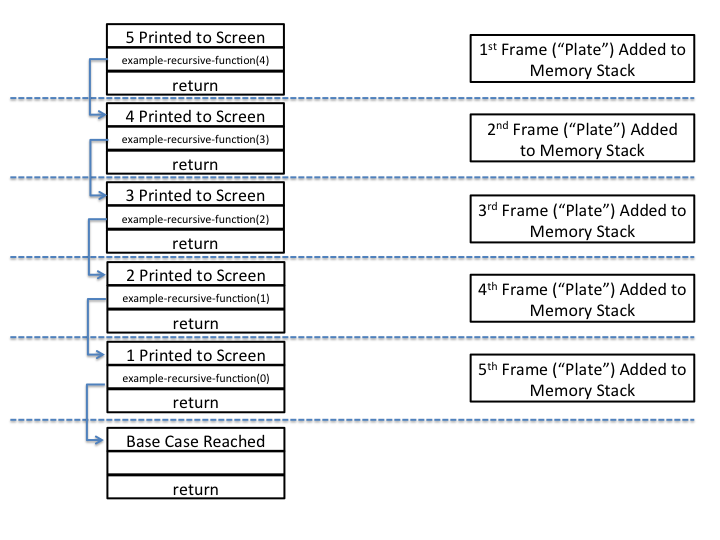
\includegraphics[height=8.5cm,keepaspectratio]{images/stack2}
\end{center}
\end{frame}

\begin{frame}
\begin{center}
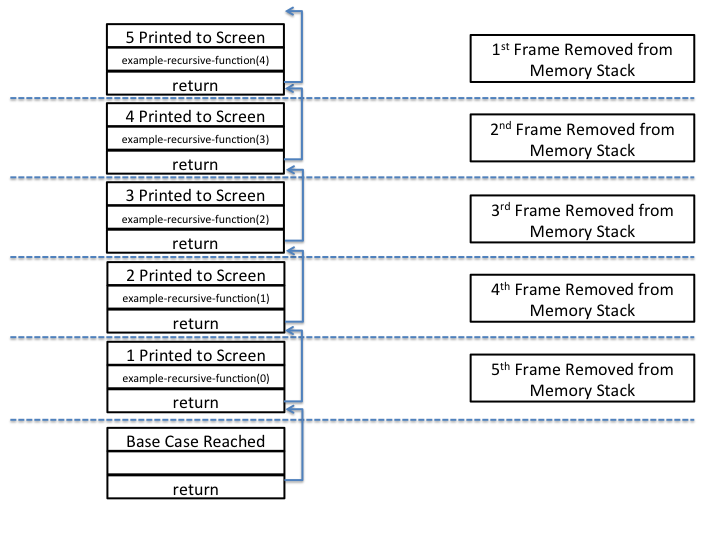
\includegraphics[height=8.5cm,keepaspectratio]{images/stack3}
\end{center}
\end{frame}

\begin{frame}[fragile]
\begin{block}{}
\begin{lstlisting}
// iterative fibonacci 
int fibonacci(int n) {
    int prev = 0;
    int curr = 1;
    int next;
    int count = 2;
    while(count <= n){
        next = prev+curr;
        prev = curr;
        curr = next;
        count = count + 1;
    }
    return curr;
}
\end{lstlisting}
\end{block}
\end{frame}

\begin{frame} 
\begin{center}
\textbf{More Examples of a WHILE Loop}
\end{center}
\begin{itemize}
\item One of the first uses of computers was to generate mathematical tables, such as log tables.
\item Table generation is a good example of iteration.
\item Over the following slides, we will develop code that prints out mathematical tables
\item We will take an incremental development approach (proposed in the lecture on incremental development) i.e.
\begin{itemize}
\item start with a main function that produces a simple output (such as a single print statement)
\item develop code gradually by adding lines
\item when it works extract it into a function
\end{itemize}
\end{itemize}
 \end{frame}

\begin{frame} 
\begin{itemize}
\item We can start with a simple main() function that calls a second create\_tables() function
\item In this first version, the create\_tables() function does nothing but print out some placeholder text
\end{itemize}
 \end{frame}
 
\begin{frame}[fragile]
\begin{block}{}
\begin{lstlisting}
#include <stdio.h>

main() 
{
    create_tables();
}

void create_tables(void)
{
    int count;
    count = 1;
    while(count < 10)
    {
        printf("placeholder\n");
        count = count + 1;
    }
}
\end{lstlisting}
\end{block}
\end{frame}

\begin{frame}
\begin{itemize}
\item We can then add a simple iteration to print out a table of logarithms
\item (base e by default) 
\end{itemize}
\end{frame}

\begin{frame}[fragile]
\begin{block}{}
\begin{lstlisting}
#include <stdio.h>
#include <math.h>

main() 
{
    create_tables();
}

void create_tables(void)
{
    int count;
    count = 1;
    while(count < 10)
    {
        double l = log(count);
        printf("%d \t %f \n",count,l);
        count = count + 1;
    }
}
\end{lstlisting}
\end{block}
\end{frame}

\begin{frame}[fragile]
\begin{block}{}
\begin{lstlisting}
$ gcc -o example_code example_code.c

$ ./example_code 
1	0.000000
2	0.693147
3	1.098612
4	1.386294
5	1.609438
6	1.791759
7	1.945910
8	2.079442
9	2.197225

\end{lstlisting}
\end{block}
\end{frame}

%% \begin{frame} 
%% \begin{itemize}
%% \item By default, the \textit{log} function uses base \textit{e}.
% % \item Since powers of two are so important in computer science, we often want to find logarithms with respect to base 2.
%\item log \textsubscript{2} \textit{x} = \textit{log}\textit{\textsubscript{e}} \textit{x} \textit{/} \textit{log }\textit{\textsubscript{e}}2
%\item One approach to calculating logarithms base 2 is, therefore to extend the program on the previous slide
%\item Once again, this follows the principle of incremental development
%\item Start with a working program and keep extending it until it does what you want it to...
%\end{itemize}
%\end{frame}
%
%
%\begin{frame}[fragile]
%\begin{block}{}
%\begin{lstlisting}
%#include <stdio.h>
%#include <math.h>
%
%main() 
%{
%    create_tables();
%}
%
%void create_tables(void)
%{
%    int count;
%    count = 1;
%    while(count < 10)
%    {
%        double l = log(count)/log(2);
%        printf("%d \t %f \n",count,l);
%        count = count + 1;
%    }
%}
%\end{lstlisting}
%\end{block}
%\end{frame}
%
%\begin{frame}[fragile]
%\begin{block}{}
%\begin{lstlisting}
%$ gcc -o example_code example_code.c
%
%$ ./example_code 
%1	0.0
%2	1.0
%3	1.584963
%4	2.0
%5	2.321928
%6	2.584963
%7	2.807355
%8	3.0
%9	3.169925
%
%\end{lstlisting}
%\end{block}
%\end{frame}
%
% \begin{frame} 
%\begin{itemize} 
%\item We can see that 1, 2, 4 and 8 are powers of two, because their logarithms base 2 are round numbers.
%\end{itemize}
%
%\begin{itemize} 
%\item Suppose we wanted to find the logarithms of other powers of two
%\item We multiply x by something, yielding a geometric sequence
%\item Once again, we can achieve this by extending our code
%\end{itemize}
% \end{frame}
%
%\begin{frame}[fragile]
%\begin{block}{}
%\begin{lstlisting}
%#include <stdio.h>
%#include <math.h>
%
%main() 
%{
%    create_tables();
%}
%
%void create_tables(void)
%{
%    int count;
%    count = 1;
%    while(count < 10)
%    {
%        double l = log(count)/log(2);
%        printf("%d \t %f \n",count,l);
%        count = count * 2;
%    }
%}
%\end{lstlisting}
%\end{block}
%\end{frame}
%
%\begin{frame}[fragile]
%\begin{block}{}
%\begin{lstlisting}
%$ gcc -o example_code example_code.c
%
%$ ./example_code
%1	0.0
%2	1.0
%4	2.0
%8	3.0
%
%\end{lstlisting}
%\end{block}
%\end{frame}

 \begin{frame} 
 \begin{center}
 \textbf{Another Example...}
 \end{center}
 
\begin{itemize}
\item The code examples on the previous slides show the utility of iteration when producing one-dimensional tables
\item Iteration is also useful when producing two-dimensional tables
\item A two-dimensional table is a table where you choose a row and a column and read the value at the intersection.
\item A multiplication table is a good example.
\end{itemize}
 \end{frame}
 
 \begin{frame}
\begin{itemize}
\item Lets print a multiplication table for the values from 1 to 6. 
\item Once again, we will build the code that produces this multiplication table step by step
\item i.e. we will use incremental development
\end{itemize}

\begin{itemize}
\item We can start with a simple loop that prints the multiples of 2 all on one line:
\end{itemize}
 \end{frame}
 
\begin{frame}[fragile] 
\begin{block}{}
\begin{lstlisting}
#include <stdio.h>

main() 
{
    create_tables();
}

void create_tables(void)
{
    int i;
    i = 1;
    while(i <= 6)
    {
        int mult = i * 2;
        printf("%d\t",mult);
        i = i + 1;
    }
}
\end{lstlisting}
\end{block}
\end{frame}


\begin{frame}[fragile] 
\begin{itemize}
\item Where:
\begin{itemize}
\item i is a counter, or loop variable. 
\item mult is the calculation want to print
\end{itemize}
\item The output of this program is:
\end{itemize}

\begin{block}{}
\begin{lstlisting}
$ gcc -o example_code example_code.c

$ ./example_code
2	4	6	8	10	12
\end{lstlisting}
\end{block}

\begin{itemize}
\item The next step is to encapsulate and generalise.  
\end{itemize}
\end{frame}

\begin{frame} 
\begin{center}
\textbf{Encapsulation and Generalisation}
\end{center}

\begin{itemize}
\item Encapsulation usually means wrapping a piece of code in a function.
\begin{itemize}
\item E.g. giving the name is\_even() to a series of statements that test whether an integer is even rather than writing
out each of those statements every time you need to run that test
\end{itemize}
\item Generalisation means taking something specific and making it more general
\begin{itemize}
\item e.g. starting with code that prints multiples of 2,
\item And changing it so that it prints multiples of any integer.
\end{itemize}
\end{itemize}

\end{frame}

\begin{frame}[fragile]
\begin{itemize}
\item Here's the previous loop as a function generalised to print multiples of any number
\end{itemize}
\begin{block}{}
\begin{lstlisting}
#include <stdio.h>

...

void print_multiples(int n)
{
    int i = 1;
    while(i <= 6)
    {
        printf("%d\t",i*n);
        i = i + 1;
    }
    printf("\n");
}
\end{lstlisting}
\end{block}

\end{frame}


\begin{frame}[fragile]
\begin{itemize}
\item print\_multiples(3) outputs:
\end{itemize}

\begin{block}{}
\begin{lstlisting}
$ ./example_code
3	6	9	12	15	18
\end{lstlisting}
\end{block}

\begin{itemize}
\item print\_multiples(4) outputs:
\end{itemize}

\begin{block}{}
\begin{lstlisting}
$ ./example_code
4	8	12	16	20	24
\end{lstlisting}
\end{block}

\end{frame}

 \begin{frame}[fragile]
\begin{itemize}
\item To print an entire multiplication table, we wrap (encapsulate) calls to print\_multiples in a loop:
\end{itemize}
\begin{block}{}
\begin{lstlisting}
#include <stdio.h>

main() 
{
    int count = 1;
    while(count < 6)
    {
        print_multiples(count);
        count = count + 1;
    }
}

... 
\end{lstlisting}
\end{block}
\end{frame}

\begin{frame}[fragile]
\begin{itemize}
\item We can now wrap (encapsulate) that encapsulation in another function
\end{itemize}

\begin{block}{}
\begin{lstlisting}
#include <stdio.h>

main() 
{
   print_tables(); 
}

void print_tables()
{
   int count = 1;
   while(count < 6)
   {
       print_multiples(count);
       count = count + 1;
   } 
}

...
\end{lstlisting}
\end{block}
\end{frame}
 
\begin{frame}[fragile]
\begin{itemize}
\item To generalise print\_tables, add a parameter
\end{itemize}

\begin{block}{}
\begin{lstlisting}
#include <stdio.h>

...

void print_tables(int high)
{
   int count = 1;
   while(count < high)
   {
       print_multiples(count);
       count = count + 1;
   } 
}

...
\end{lstlisting}
\end{block}
\end{frame}

\begin{frame}[fragile]
\begin{itemize}
\item If printTable is called with the argument 7, we get the following output
\end{itemize}

\begin{block}{}
\begin{lstlisting}
$ ./example_code
1	2	3	4	5	6	
2	4	6	8	10	12	
3	6	9	12	15	18	
4	8	12	16	20	24	
5	10	15	20	25	30	
6	12	18	24	30	36
\end{lstlisting}
\end{block}
\end{frame}


\begin{frame}[fragile]
\begin{block}{}
\begin{lstlisting}
#include <stdio.h>

main() 
{
   print_tables(7); 
}

void print_tables(int high)
{
   int count = 1;
   while(count < high)
   {
       print_multiples(count);
       count = count + 1;
   } 
}

...
\end{lstlisting}
\end{block}
\end{frame}

\begin{frame}[fragile]
\begin{block}{}
\begin{lstlisting}
... 

void print_multiples(int n)
{
    int i = 1;
    while(i <= 6)
    {
        printf("%d\t",i*n);
        i = i + 1;
    }
    printf("\n");
}
\end{lstlisting}
\end{block}
\end{frame}

% \begin{frame}
% \begin{center}
% \textbf{Exercises}
% \end{center}
% \begin{itemize}
% \item \textbf{Exercise 1}: In groups of 2-3 draw a diagram of the flow of control through this code
% \item \textbf{Exercise 2}: In the  same groups, decide where you would put print statements in order to check that the  flow of control is passing as  you expect
% \item \textbf{Exercise 3}: Spend 5 minutes writing down the output you expect from those print statements for each pass through the  three methods in the code 
% \end{itemize} 
% \end{frame}
 
\begin{frame} 
\begin{center}
\textbf{Next Steps}
\end{center}
\begin{itemize}
\item The code we have written so far prints the results of our calculations to the standard out
\item However, we might want to save these results for future use
\item One way to do this in C is by using an Array 
\item Arrays are a common data structure in all programming languages
\end{itemize}
 \end{frame}
 
\begin{frame} 
\begin{center}
\textbf{Arrays}
\end{center}
\begin{itemize}
\item You can recognise an array in a C program by the appearance of square brackets   [  ]
\item An array is a container that holds a fixed number of values of a single type e.g.
\begin{itemize}
\item 9 ints e.g. [1, 2, 300, 4, 500, 6, 7, 800, 9]
\item 4 chars e.g. [a, z, e, g]
% \item 2 booleans e.g. [true, true]
\end{itemize}
\end{itemize}
 \end{frame}
 
 \begin{frame} 
\begin{itemize}
\item Each item within an array is called an \textbf{element }
\item Each element is referred to by its numerical \textbf{index}
\begin{itemize}
\item The first element in an array is referred to as \textbf{[ 0 ]}
\item The second element is referred to as \textbf{[ 1 ]}
\item The third element is referred to as \textbf{[ 2 ]}
\item and so on ...
\end{itemize}
\end{itemize}
 \end{frame}

\begin{frame}[fragile]
\begin{itemize}
% \item Once again, we will build the code to achieve storage of our mathematical table in an incremental manner
\item In C a one dimensional array (a series of values) is declared
\end{itemize}

\begin{block}{}
\begin{lstlisting}
int an_array[7];
\end{lstlisting}
\end{block}

\begin{itemize}
\item Note: You have to allocate memory for the number of elements that you want to exist in that array before you can store data within it
\end{itemize}
\end{frame}

\begin{frame}[fragile]
\begin{itemize}
\item Any expression with type \textbf{int} can be used as an index.
\end{itemize}

\begin{block}{}
\begin{lstlisting}
an_array[7-5];
\end{lstlisting}
\end{block}

\begin{itemize}
\item Other data types may \textbf{not} be used as an index
\end{itemize}

\begin{block}{}
\begin{lstlisting}
an_array[2.0];   /* ERROR */
\end{lstlisting}
\end{block}

\begin{itemize}
\item If you refer to an element that does not exist, you will get an error.
\end{itemize}

\begin{block}{}
\begin{lstlisting}
int an_array[5];
an_array[20] = 21;   /* ERROR */
\end{lstlisting}
\end{block}
\end{frame}

\begin{frame}
\begin{itemize}
\item Correct referencing is, perhaps more easily understood through use of an example
\end{itemize}
\begin{itemize}
\item The following code sets up an array of integers ...
\item ... and assigns a value to each element in the array
\end{itemize}
 \end{frame}

\begin{frame}[fragile]
\begin{block}{}
\begin{lstlisting}
#include <stdio.h>

main() 
{
    int myarray[5];
    myarray[0] = 1;
    myarray[1] = 2;
    myarray[2] = 3;
    myarray[3] = 4;
    myarray[4] = 5;
}
\end{lstlisting}
\end{block}
\end{frame}

\begin{frame}[fragile]
\begin{itemize}
\item We can now print data held in the array as we would any other variable
\end{itemize}

\begin{block}{}
\begin{lstlisting}
printf("%d\t",myarray[2]);
\end{lstlisting}
\end{block}

\begin{itemize}
\item We can also assign the value held in an array element to another variable
\end{itemize}
\begin{block}{}
\begin{lstlisting}
int y = myarray[2];
printf("%d\t",y);
\end{lstlisting}
\end{block}
\end{frame}
 
\begin{frame}[fragile]
\begin{itemize}
\item In C you can also declare two-dimensional (e.g. 2x2) arrays
\end{itemize}

\begin{block}{}
\begin{lstlisting}
#include <stdio.h>

main() 
{
    int myarray[2][2];
    myarray[0][0] = 1;
    myarray[0][1] = 2;
    myarray[1][0] = 3;
    myarray[1][1] = 4;
}
\end{lstlisting}
\end{block}
\end{frame}

 \begin{frame} 
\begin{itemize}
\item We now have all of the C language structures that we need to store the output of print\_tables in a two-dimensional array
\item Actually writing that code will be one of your lab exercises so I will not go through the answer in these  slides
\end{itemize}
 \end{frame}
 
 \begin{frame}
\begin{itemize}
\item Be aware that this last step in our incremental development exercise is not as easy as it looks
\item You may find it helpful to reconsider the number of methods that you implement when developing this storage function
\item Remember to take an incremental approach to building your programs
\item That is, start with a program that works and then extend it
\item If you get stuck, ask the tutors for help!
\end{itemize}
 \end{frame}

\section{Strings}
\begin{frame}
\begin{itemize}

\item {\color{black}
In the first two weeks of the course, we have looked at different ways to describe data}
\item {\color{black}
More specifically, we have seen the importance in C of describing the type of the data that we store and use.}

\begin{itemize}
\item {\color{black}
e.g. ints, chars, floats, doubles and booleans}
\end{itemize}
\item {\color{black}
Assigning types }

\begin{itemize}
\item {\color{black}
Helps the compiler to know how much memory to allocate and}
\item {\color{black}
Can also be used to limit the computations on each piece of data to those that are relevant to data of each type}
\end{itemize}
\end{itemize}
\end{frame}


\begin{frame}
\begin{itemize}
\item {\color{black}
In the previous section of these slides, we also looked at collecting data in an Array}
\item {\color{black}
For the remainder of this week and the first part of next, we will look the ways in which C uses Arrays to underpin another very common data type: Strings }
\end{itemize}
\end{frame}


\begin{frame}
\begin{itemize}

\item {\color{black}
Strings in C are stored as an array of chars}
\item {\color{black}
More specifically, a string (in C) is a one dimensional array of chars terminated by a null character
('{\textbackslash}0')}
\item {\color{black}
So a String containing the single word ``Hello'' is actually a six char array (5 letters and a null character).}

\end{itemize}
\end{frame}


\begin{frame}
\begin{itemize}
\item A variable containing the String ``Hello'' can be declared and initialised in multiple ways
\end{itemize}
\end{frame}

\begin{frame}[fragile]
\begin{itemize}
\item The long version mirrors the ways in which we populated arrays earlier
\end{itemize}

\begin{block}{}
\begin{lstlisting}
char greeting[6];

greeting[0] = 'H';
greeting[1] = 'e';
greeting[2] = 'l';
greeting[3] = 'l';
greeting[4] = 'o';
greeting[5] = '\0';

\end{lstlisting}
\end{block} 
\end{frame}


\begin{frame}[fragile]
\begin{itemize}

\item {\color{black}
A slightly shorter version is as follows:}

\begin{block}{}
\begin{lstlisting}

char greeting[6] = {'H', 'e', 'l', 'l', 'o', '\0'};

\end{lstlisting}
\end{block} 

\end{itemize}
\end{frame}

\begin{frame}[fragile]

\begin{itemize}
\item {\color{black}
In C, you can also declare and initialise an Array of characters with a String literal (a special case):}
\end{itemize}

\begin{block}{}
\begin{lstlisting}
char greeting[] = "Hello";
\end{lstlisting}
\end{block} 

\begin{itemize}
\item {\color{black}
Note in this case that the compiler adds the null character ('{\textbackslash}0') for you.}
\end{itemize}
\end{frame}

\begin{frame}[fragile]
\begin{itemize}

\item {\color{black}
Be careful when using this special case, however since neither of the two following approaches is permitted:}

\begin{block}{}
\begin{lstlisting}

char greeting[];	
greeting = “Hello”;		//syntax error

char greeting2[12];
greeting2 = “Hello Again”;	//also a syntax error

\end{lstlisting}
\end{block}

\end{itemize}
\end{frame}

\begin{frame}
\begin{itemize}
\item An aside: Just as Arrays are stored as Arrays of chars in C,
\item chars themselves are actually stored as as unsigned integers
\item i.e. an int code is used to represent each char e.g.
\item 97 is the code used to represent the char 'a'

\item 113 is the code used to represent the char 'q'
\item 65 is the code used to represent the char 'A'
\end{itemize}
\end{frame}

\begin{frame}
\begin{itemize}
\item NOTE\\: Upper case characters are associated with different codes than their lower case equivalents
\item NOTE\\: and special characters like '\&' also have codes associated with them (38)
\item more detail on the American Standard Codes for Information Interchange (ASCII) can be found online
\item e.g. http://web.cs.mun.ca/~michael/c/ascii-table.html

\end{itemize}
\end{frame}

\begin{frame}[fragile]
\begin{itemize}
\item One implication of the way in which C stores chars is that we can also declare and initialise the String "Hello" as follows
\end{itemize}

\begin{block}{}
\begin{lstlisting}
char greeting[6];

greeting[0] = 72;
greeting[1] = 101;
greeting[2] = 108;
greeting[3] = 108;
greeting[4] = 111;
greeting[5] = 0;

\end{lstlisting}
\end{block} 
\end{frame}


\begin{frame}[fragile]
\begin{itemize}
\item {\color{black}
Once we have created Strings use any of the approaches above, we can print them using printf() as before e.g.:}
\end{itemize}

\begin{block}{}
\begin{lstlisting}

#include <stdio.h>

int main ()
{
   char greeting[6] = {'H', 'e', 'l', 'l', 'o', '\0'};

   printf("Greeting message: %s\n", greeting );

}

\end{lstlisting}
\end{block}

\begin{block}{}
\begin{lstlisting}

$ Greeting message: Hello

\end{lstlisting}
\end{block}

\begin{itemize}
\item {\color{black}
Note the use of a new format specifier, \%s for Strings }

\end{itemize}
\end{frame}

\begin{frame}[fragile] 
\begin{itemize}
\item Just like the other C data types that we have looked at, strings can be...
\end{itemize}

\begin{itemize}
\item ... assigned to variables
\end{itemize}
\begin{block}{}
\begin{lstlisting}
char my_string[] = "hello world";
\end{lstlisting}
\end{block} 

\begin{itemize}
\item ... passed to methods as parameters
\end{itemize}
\begin{block}{}
\begin{lstlisting}
void print_string(char a_string[])
{
    printf(a_string);   
}  
\end{lstlisting}
\end{block} 
\end{frame}


\begin{frame}[fragile]
\begin{itemize}

\item {\color{black}
We can manipulate individual chars in a String, just as we manipulated the individual integers in
the multiplication arrays introduced earlier:}

\end{itemize}
\end{frame}

\begin{frame}[fragile]

\begin{block}{}
\begin{lstlisting}
#include <stdio.h>

int main ()
{
   char greeting[6] = {'H', 'e', 'l', 'l', 'o', '\0'};
    greeting[1]='o';
    greeting[2]='w';	
    greeting[3]='d';
    greeting[1]='y';
   printf("Greeting message: %s\n", greeting );	
    printf("First letter is: %c\n", greeting[0]);	
}

\end{lstlisting}
\end{block}

\begin{block}{}
\begin{lstlisting}
Greeting message: Howdy
First letter is: H

\end{lstlisting}
\end{block}
\end{frame}

\begin{frame}[fragile]
\begin{itemize}

\item {\color{black}
In addition to the standard array functions, including string.h in a C program provides support for a wide range of
functions that manipulate null-terminated strings e.g.:}

\begin{itemize}
\item {\color{black}
strcpy(s1,s2) copies string s2 into s1}
\item {\color{black}
strcat(s1,s2) Concatenates (adds) string s2 onto the send of string s1}
\item {\color{black}
strlen(s1) returns the length of string s1 as an integer}
\end{itemize}
\end{itemize}
\begin{itemize}
\item \textcolor{black}{The f}\textcolor{black}{ollowing example makes use of few of the above-mentioned functions:}
\end{itemize}
\end{frame}

\begin{frame}[fragile]
\begin{block}{}
\begin{lstlisting}
#include <stdio.h>
#include <string.h>

int main ()
{
   char str1[12] = "Hello";
   char str2[12] = "World";
   char str3[12];		
   int  len ;
 
   strcpy(str3, str1); /* copy str1 into str3 */
   printf("strcpy( str3, str1) :  %s\n", str3 );

   strcat( str1, str2); /* concatenate str1 & str2 */
   printf("strcat( str1, str2):   %s\n", str1 );
  
   len = strlen(str1); /* length of str1 */
   printf("strlen(str1) :  %d\n", len );
   return 0;
}

\end{lstlisting}
\end{block}

\begin{block}{}
\begin{lstlisting}

strcpy( str3, str1) :  Hello
strcat( str1, str2):   HelloWorld
strlen(str1) :  10

\end{lstlisting}
\end{block}
\end{frame}

\begin{frame}[fragile]
\begin{itemize}
\item Using a combination of strlen() and iteration, we can print out each char in a string on a separate line
\end{itemize}
\begin{block}{}
\begin{lstlisting}
void print_string(char a_string[])
{
    int i = 0;
    while (i < strlen(a_string)){
        printf("%c\n", a_string[i]);
        i++;
    }
}
\end{lstlisting}
\end{block}
\end{frame}

\begin{frame}[fragile]
\begin{itemize}
\item strlen will return how many elements are in the string
\item But remember to access arrays we start counting from 0
\item The WRONG way to find the last letter of a string:
\end{itemize}
\begin{block}{}
\begin{lstlisting}
char my_string[] = "Hello World";
int i = strlen(my_string);
printf("%c\n",my_string[i]);   /* ERROR!! */
\end{lstlisting}
\end{block}
\begin{itemize}
\item Remember that the first character in a string has index 0 so the correct code would be:
\begin{block}{}
\begin{lstlisting}
char my_string[] = "Hello World";
int i = strlen(my_string);
printf("%c\n",my_string[i-1]); 
\end{lstlisting}
\end{block} 
\end{itemize}
\end{frame}

\begin{frame}[fragile]
\begin{itemize}
\item A common computation to perform on a string (or any collection of data) is start at the beginning, select each character (element) in turn, do something to it (e.g. print it), and continue until the end.
\item This pattern of processing is called a traversal.
\item We saw how to do this with a while loop on a previous slide
\end{itemize}
\begin{block}{}
\begin{lstlisting}
void print_string(char a_string[])
{
    int i = 0;
    while (i < strlen(a_string)){
        printf("%c\n", a_string[i]);
        i++;
    }
}
\end{lstlisting}
\end{block}
\end{frame}

\begin{frame}[fragile]
\begin{itemize}
\item We can also achieve that traversal by using a for loop: 
\end{itemize}

\begin{block}{}
\begin{lstlisting}
void print_string(char a_string[])
{
   char my_string[] = "Hello World";
   int i;
   for(i=0; i<strlen(my_string);i++)
   {
        printf("%c\n", my_string[i]);
   } 
}
\end{lstlisting}
\end{block}
\end{frame}

\begin{frame}[fragile]
\begin{itemize}
\item The structure of a for loop is as follows:
\end{itemize}
\begin{block}{}
\begin{lstlisting}
for (initialization; termination; increment) 
{
	statement 1
	statement 2
	statement n
}
\end{lstlisting}
\end{block}
\end{frame}

\begin{frame}
\begin{itemize}
\item Note, however, that those examples have been carefully chosen
\item We have not tried to put Strings into Arrays that are not long enough to hold them 
\item i.e. we have been very careful to limit the number of characters that we copy into a target string or concatenate
onto the end of it to respect the number of characters that the target string can hold
\item (We have on occasion left space unused at the end of an Array [e.g. created an Array that can hold 12 elements and used only six to store ``Hello''])
\end{itemize}
\end{frame}

\begin{frame}
\begin{itemize}
\item To create exactly the right amount of memory to hold Strings at runtime, we have to understand the way that C handles the memory associated with those arrays
\item we will return to that subject next week

\end{itemize}
\end{frame}

\begin{frame}[fragile]
\begin{itemize}

\item It is, however, worth noting an special use of Strings in C:
\item More specifically, it is worth noting that we can send one or more Strings to our main method when running a
program.
\end{itemize}
\end{frame}


\begin{frame}[fragile]
\begin{itemize}

\item In previous exercises, you have been using gcc(with or without flags and specified output files) \ to compile your C code 
\item and used only the name of the output file to run that compiled code e.g.


\begin{block}{}
\begin{lstlisting}
$ gcc HelloWorld.c
$ a.out

\end{lstlisting}
\end{block}

\end{itemize}
\end{frame}

\begin{frame}
\begin{itemize}


\item We can, however pass a string to the HelloWorld program at the point of running it and use that String within the
main method
\item In order to do so, however, we would need to add instructions to the main method to do exactly that

\end{itemize}
\end{frame}

\begin{frame}
\begin{itemize}

\item More specifically, we need to specify two parameters ("arguments") in the main method

\begin{itemize}
\item int argc which describes the number of Strings passed as input plus one (since the name of the program is also
counted)
\item int *argv which holds the Strings themselves (the program name is held in argv[1]
\end{itemize}
\item an argument introduced at the command line is (unsurprisingly) referred to as a command line argument

\end{itemize}
\end{frame}

\begin{frame}[fragile]
\begin{block}{}
\begin{lstlisting}

/* Original Hello World program */
#include<stdio.h>
main()
{
 printf("Hello World");
}

\end{lstlisting}
\end{block}

\begin{block}{}
\begin{lstlisting}

$ gcc HelloWorld.c
$ a.out
Hello World

\end{lstlisting}
\end{block}

\end{frame}


\begin{frame}[fragile]
\begin{block}{}
\begin{lstlisting}
/* 
* HelloWorld 
* extended to take a command line single argument 
* and print it to the screen
* At this point, dont worry about the * preceding argv
*/
#include <stdio.h>
int main( int argc, char *argv[] )  
{
     printf("The number of arguments passed is %d\n", argc-1);
     printf("The name of your program is %s\n", argv[0]);
     printf("The argument supplied is %s\n", argv[1]);
}
\end{lstlisting}
\end{block}
\end{frame}

\begin{frame}[fragile]
\begin{block}{}
\begin{lstlisting}

$ gcc HelloWorld.c
$ a.out testing
The number of arguments supplied is 1
The argument supplied is testing

\end{lstlisting}
\end{block}
\end{frame}


\begin{frame}
\begin{itemize}
\item NOTE: we can pass multiple command line aguments
\item if we had passed a second argument (a Second String) it would now be held in argv[2]
\item and the (int) value held in argc would be 3
\end{itemize}
\end{frame}


\begin{frame}[fragile]
\begin{block}{}
\begin{lstlisting}
/*
* HelloWorld with guards
*/
#include <stdio.h>
int main( int argc, char *argv[] )  
{
   if( argc == 2 )
   {
     printf("The argument supplied is %s\n", argv[1]);
     printf("The argument's first letter is %c\n", argv[1][0]);
   }
   else if( argc > 2 )
   {
     printf("Too many arguments supplied.\n");
   }
   else
   {
     printf("One argument expected.\n");
   }
}
\end{lstlisting}
\end{block}
\end{frame}


\begin{frame}[fragile]
\begin{block}{}
\begin{lstlisting}

$ gcc HelloWorld.c
$ a.out testing
The argument supplied is testing
The arguments first letter t

\end{lstlisting}
\end{block}
\end{frame}

\begin{frame}
\begin{itemize}
\item NOTE: Do not worry if you do not fully understand the "HelloWorld with guards" code on the previous slides
\item We will return to it next week
\item For now, just be aware that it gives you example code that you can use to take a command line argument and print it to screen
\item remember the incremental programming approach - start with something that works and add to (or subtract from) it
\end{itemize}
\end{frame}
\end{document}